% C.28 ⊙O，∠AOB=80°，C 在优弧上
\documentclass[tikz,border=4pt]{standalone}
\usepackage{ctex}
\usepackage{amsmath}
\usetikzlibrary{calc, arrows.meta}
\begin{document}
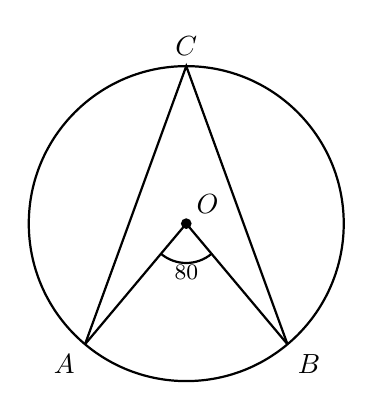
\begin{tikzpicture}[scale=1.0, thick]
  \coordinate (O) at (0,0);
  \draw (O) circle (2);
  \coordinate (A) at ({2*cos(-130)}, {2*sin(-130)});
  \coordinate (B) at ({2*cos(-50)}, {2*sin(-50)});
  \coordinate (C) at (0,2);
  \draw (O) -- (A);
  \draw (O) -- (B);
  \draw (A) -- (C) -- (B);
  \filldraw (O) circle (1.5pt) node[above right] {$O$};
  \node[below left] at (A) {$A$};
  \node[below right] at (B) {$B$};
  \node[above] at (C) {$C$};
  \draw ({0.5*cos(-130)},{0.5*sin(-130)}) arc (-130:-50:0.5);
  \node[font=\footnotesize, below] at (0,-0.4) {$80°$};
\end{tikzpicture}
\end{document}
